% ch01g: 第 1 章附录 A–F（印刷页 52–63，§1.9–§1.14）

\section{附录 A：X 型的簇代数簇}

这里我们汇集 X 型簇代数簇所需的定义与性质。为简便起见，我们只限于所谓的单链情形，此时交换矩阵是斜对称的。

种子环面不过是一对 $(\mathcal{X},\varepsilon)$，其中 $\mathcal{X}=(\C^\times)^N$ 是可裂代数环面，$\varepsilon^{ij}$（$1\leqslant i,j\leqslant N$）是一个称为交换矩阵的斜对称矩阵。$\mathcal{X}$ 上的标准坐标记作 $\{x_i\}$。两个种子环面 $(\mathcal{X},\varepsilon)$ 与 $(\mathcal{X}',\varepsilon')$ 之间的同构，是保持这种分裂、并把一个交换矩阵送到另一个交换矩阵的映射；它由坐标集合的一个双射 $\sigma\colon\{1,\dots,N\}\to\{1,\dots,N\}$ 给出，使得 $\varepsilon^{ij}=\varepsilon'_{\sigma(i)\sigma(j)}$。

两个种子 $(\mathcal{X},\varepsilon)$ 与 $(\mathcal{X}',\varepsilon')$ 之间在第 $k$ 个坐标上的一个变异，是一个映射，它满足 $\varepsilon^{ik}\in\Z$（对任意 $i$），把交换矩阵按
\[
\varepsilon'_{ij}=
\begin{cases}
-\varepsilon^{ij}, & \text{若 } i=k \text{ 或 } j=k,\\
\varepsilon^{ij}, & \text{若 } \varepsilon^{ik}\varepsilon^{kj}<0,\\
\varepsilon^{ij}+\varepsilon^{ik}|\varepsilon^{kj}|, & \text{其余情形}
\end{cases}
\]
相联系，并把坐标按
\[
x'_i=
\begin{cases}
1/x_i, & \text{若 } i=k,\\
x_i(1+x_k)^{\varepsilon^{ij}}, & \text{若 } \varepsilon^{ij}\geqslant 0,\\
x_i(1+1/x_k)^{\varepsilon^{ij}}, & \text{若 } \varepsilon^{ij}<0
\end{cases}
\]
相联系。\begin{annote}底本此处把 $x'_i$ 的指数以及分情形所依据的符号都写成 $\varepsilon^{ij}$。但第 $k$ 个坐标上的变异只应涉及联系 $i$ 与 $k$ 的矩阵元，此处疑为笔误；译文照底本排印。[来源：上下文推断]\end{annote}

簇变换是若干个变异的复合；簇映射是若干个簇变换与沿标准坐标轴的投影的复合。

X 型的簇代数簇是一个代数簇，它在余维二的意义下被一族（可能无限的）簇坐标卡所覆盖。这些坐标卡是映射 $\varphi^\alpha\colon\mathcal{X}^\alpha\to X$，其中 $\{(\mathcal{X}^\alpha,\varepsilon^\alpha)\}$ 是一族种子，并且任何转移函数 $(\varphi^\alpha)^{-1}\circ\varphi^\beta$ 都是簇变换。簇代数簇带有典范的 Poisson 结构，它在任何簇坐标卡 $(\mathcal{X}^\alpha,\varepsilon^\alpha)$ 中由
\begin{equation}
\{x_i,x_j\}=\varepsilon^{ij}x_ix_j
\tag{1.57}
\label{eq:1.57}
\end{equation}
给出。

$X$ 上的一个正则函数，若在任何坐标卡中都是系数为正整数的 Laurent 多项式，则称为簇函数。不能写成两个簇函数之和的簇函数称为不可分解的。猜想：不可分解的簇函数的集合构成 $X$ 上正则函数空间的一组基。这组基称为典范基。

为在两个簇代数簇 $X$ 与 $Y$ 之间构造一个（双有理）同构，只需构造 $X$ 的一个种子与 $Y$ 的一个种子之间的同构。特别地，一个种子与由它经簇变换得到的种子之间的任何同构，都定义了整个簇代数簇的一个自同构。这类变换构成的群称为簇代数簇 $X$ 的映射类群。这个名称来自与 Teichmüller 理论的类比：在 Teichmüller 理论中，这个群确实是相应曲面的映射类群；但在我们这里不应按字面理解这个名称。

\section{附录 B：单链李群的生成元之间的关系}

\begin{enumerate}[label=(\roman*),leftmargin=3em,itemsep=2pt]
\item $H_i(x)H_j(y)=H_j(y)H_i(x)$，
\item $H_i(x)H_i(y)=H_i(xy)$，
\item $E_iH_i(-1)E_i=H_i(-1)$，
\item 当 $i\neq|j|$ 时，$H_i(x)E_j=E_jH_i(x)$，
\item 若 $C_{ij}=0$，则 $E_iE_j=E_jE_i$，
\item $E_iH_i(x)E_i=H_i(1+x)E_iH_i(1+x^{-1})^{-1}$，
\item 若 $C_{ij}=-1$ 且 $i,j>0$，则
\[
\begin{aligned}
E_iH_i(x)E_jE_i={}&H_i(1+x)H_j(1+x^{-1})^{-1}E_jH_j(x)^{-1}E_iE_jH_i(1+x^{-1})^{-1}\\
&\cdot H_j(1+x),
\end{aligned}
\]
\item 若 $C_{ij}=-1$ 且 $i,j>0$，则
\[
\begin{aligned}
E_{\bar\imath}H_i(x)E_{\bar\jmath}E_{\bar\imath}={}&H_i(1+x^{-1})^{-1}H_j(1+x)E_{\bar\jmath}H_j(x)^{-1}E_{\bar\imath}E_{\bar\imath}H_i(1+x)\\
&\cdot H_j(1+x^{-1})^{-1},
\end{aligned}
\]
\item 当 $i>0$ 时，
\[
E_{\bar\imath}H_i(x)E_i=\prod_{j\neq i}H_j(1+x)^{-C_{ij}}H_i(1+x^{-1})^{-1}E_iH_i(x^{-1})E_{\bar\imath}H_i(1+x^{-1})^{-1}.
\]
\end{enumerate}
\begin{annote}第 (viii) 式右端中部出现因子 $E_{\bar\imath}E_{\bar\imath}$，而按第 (vii) 式的模式此处应为 $E_{\bar\imath}E_{\bar\jmath}$。底本如此排印，译文照排。[来源：上下文推断]\end{annote}

\section{附录 C：交换图与 \texorpdfstring{$u\in W\times W$}{u ∈ W×W} 的分解}

如 [4] 所示，由 Drinfeld--Jimbo $r$-矩阵 (1.2) 在参数 $x_i$ 上诱导的 Poisson 括号是对数常值的，且取半整数值；也就是说，它由公式 (1.57) 给出，其中 $\varepsilon^{ij}$ 是取整数值或半整数值的斜对称矩阵。同一个矩阵（当群 $G$ 单链时）扮演相应簇代数簇的交换矩阵的角色。下面我们描述 §1.3 与 §1.4 中所用的胞腔参数化对应的矩阵 $\varepsilon^{ij}$。

我们不去写出公式，而是构造一个带定向边的图，称为交换图（exchange graph）\footnote{这个图与环面 $\Sigma$ 上用来构造二聚体配分函数的二部图 $\Gamma$ 对偶。}：它的顶点与指标 $i$（或相应的坐标函数 $x_i$）一一对应；当 $\varepsilon^{ij}\geqslant 0$ 时，从 $i$ 到 $j$ 有 $\varepsilon^{ij}$ 条箭头。若 $\varepsilon^{ij}$ 取半整数值，其小数部分用灰色箭头表示，见图 1.20 与图 1.21。

设 $u=s_{k_1}\cdots s_{k_l}$ 是由 $W\times W$ 的生成元作成的词。为构造这个图，先取一个谱表（staff），即平面上一族互不相交的水平线，按正单根 $i\in\Pi$ 列举。谱表上的点按其水平投影排序，如同音乐记谱中那样。对每个 $k_j$ 画一条弦，即一个图 $\Gamma(k_j)$，其顶点在谱表上，边带定向。不同的弦按生成元 $s_{k_j}$ 在词中的顺序放在谱表上，例如弦 $\Gamma(k_{j+1})$ 位于弦 $\Gamma(k_j)$ 的右边。

弦 $\Gamma(k_j)$ 在第 $j$ 条线（$j\in\Pi$）上有最左顶点 $L_j(k_j)$ 与最右顶点 $R_j(k_j)$；在其余每条线上、位于 $L_j(k_j)$ 与 $R_j(k_j)$ 之间还有顶点 $\{S_l(k_j)\mid l\neq j\}$，它们的相互顺序是任意的。若 $k_j>0$，我们在谱表第 $j$ 条线上、$L_j(k_j)$ 与 $R_j(k_j)$ 之间画一条前向定向的边，并用 $-C_{jl}/2$ 条后向定向的边把 $L_j(k_j)$ 与 $R_j(k_j)$ 同 $S_l(k_j)$ 相连（大多数情形下画成灰色，表示 $-C_{jl}/2$ 常常等于 $1/2$）。若 $k_j<0$，我们画同样的弦，但所有箭头的定向相反，见图 1.20 与图 1.21 的左图。

\begin{figure}[htbp]
\centering
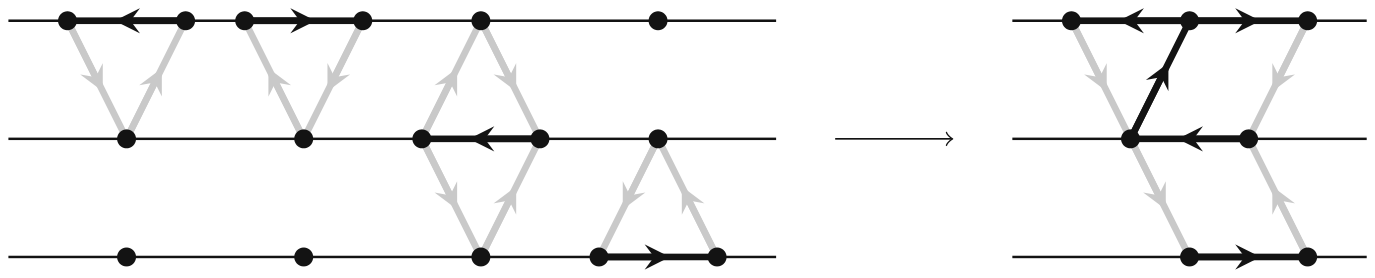
\includegraphics[width=363.0pt]{figs/f1-20.png}
\caption{左：对词 $\bar1123$，由一串有序的弦构成的图之例，情形为 $\operatorname{PGL}(4)$。右：把它粘合为单个图的结果。}
\label{fig:1.20}
\end{figure}

\begin{figure}[htbp]
\centering
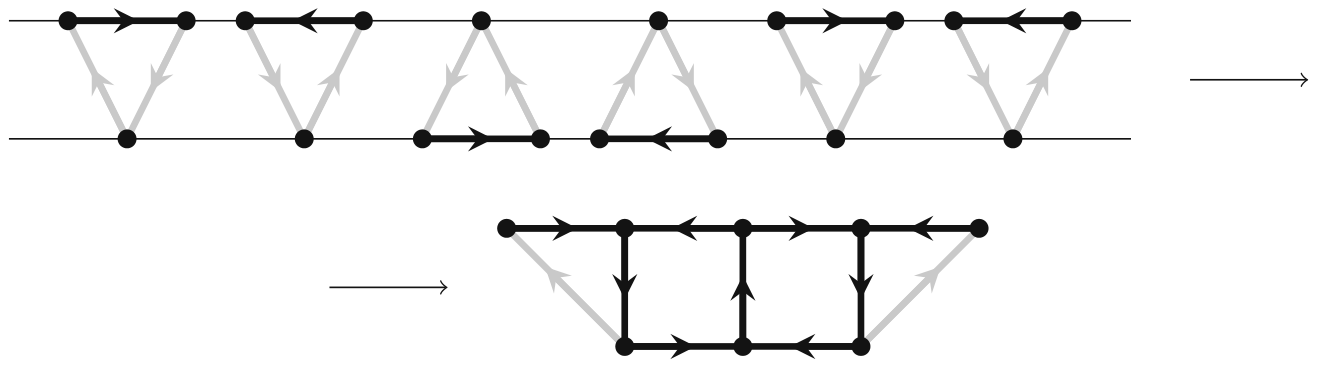
\includegraphics[width=347.7pt]{figs/f1-21.png}
\caption{对词 $1\bar12\bar21\bar1$（大胞腔），按图 1.20 的方式由粘合的弦构造出的图之例，群为 $\operatorname{PGL}(3)$。}
\label{fig:1.21}
\end{figure}

要得到所求的图，只需把所有谱表线收缩掉，并删去连接同一对顶点、方向相反的那些箭头对，如图 1.20 与图 1.21 的右图所示。图 1.21 中的图恰好对应于我们上面考虑过的 $\operatorname{PGL}(3)$ 中大胞腔的例子（见 §1.3 中的公式 (1.10)）。

为构造商 $G/\operatorname{Ad}H$ 的胞腔所对应的图，只需把谱表放在柱面上而不是平面上，于是谱表线变成圆圈。例如，$\operatorname{PGL}(3)/\operatorname{Ad}H$ 中对应于图 1.21 的辛叶的图，可以通过把每条谱表线的最左点与最右点等同起来得到。类似地，$\operatorname{PGL}(3)$ Toda 链的辛叶所对应的图（比较 (1.11)）完全同样地构造，见图 1.22。

\begin{figure}[htbp]
\centering
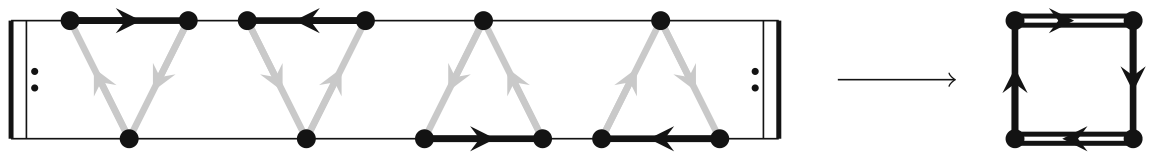
\includegraphics[width=304.7pt]{figs/f1-22.png}
\caption{对词 $\bar11\bar22$，群为 $\operatorname{PGL}(3)/\operatorname{Ad}H$ 的交换图之例。}
\label{fig:1.22}
\end{figure}

\section{附录 D：Thurston 图}
定向曲面 $\Sigma$ 上的一个 Thurston 图，是一族定向曲线的同痕类，使得所有交点都是三重点，并且在每个交点处曲线的定向是交错的。圆盘上的一个 Thurston 图之例见图 1.23 A。曲线既可以是闭的，也可以从边界走到边界。曲线补集的连通分支称为面。交点处的定向条件意味着：围成一个面的那些曲线段的定向要么是顺时针的（此时该面称为白面），要么是逆时针的（此时该面称为灰面）。与白面相邻的面都是灰面，反之亦然。在图中我们不标出曲线的定向，因为它们可以由面的着色恢复。

Thurston 图容许四种标准修改，见图 1.24 A、B、C、D。前两种称为 Thurston 变换，它们不改变面的个数；后两种减少面的个数，称为 Thurston 约化。每当出现有一个或两个角的面时，就可以施行一次变换；由 Thurston 变换相联系的图称为等价的。若一个图不等价于任何可以施行 Thurston 约化的图，则称它为极小的。

\begin{figure}[htbp]
\centering
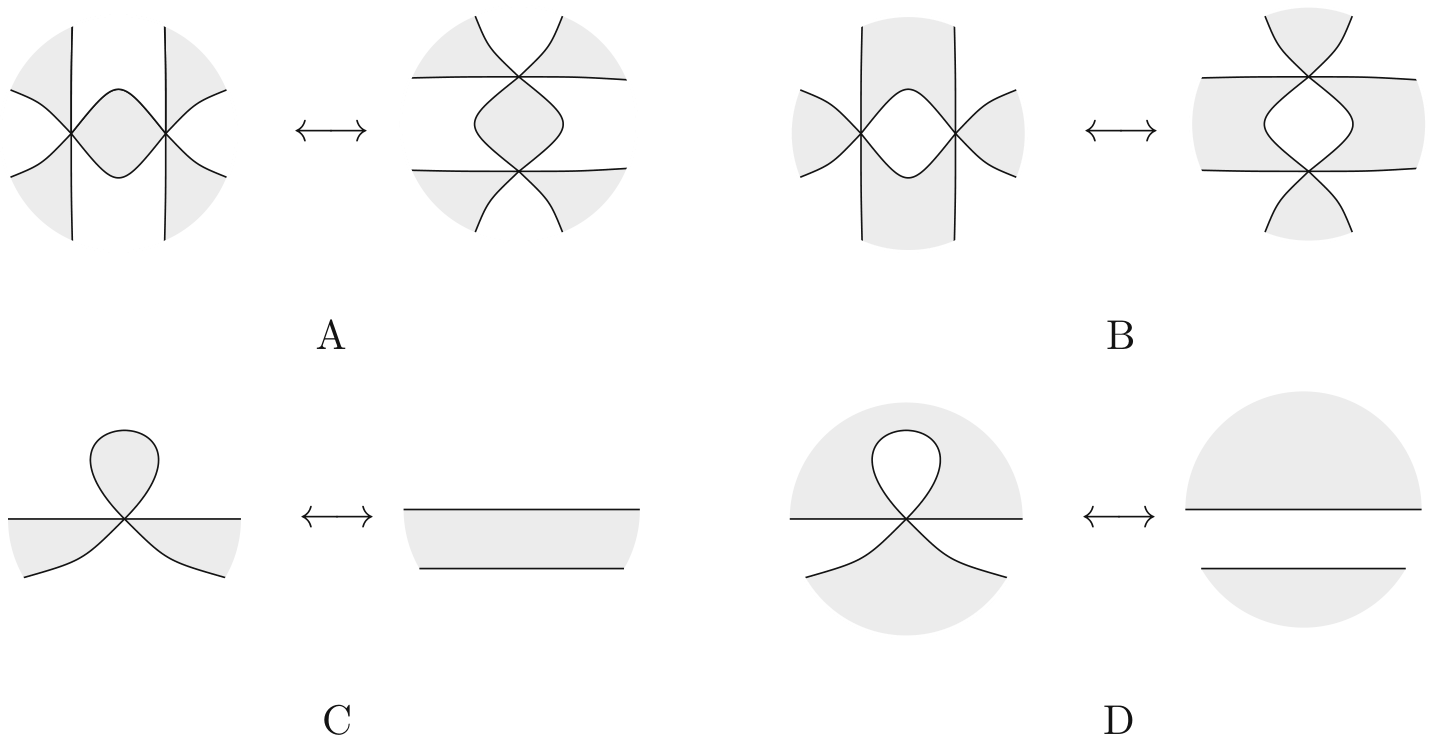
\includegraphics[width=378.3pt]{figs/f1-24.png}
\caption{A：灰色 Thurston 变换；B：白色 Thurston 变换；C：灰色 Thurston 约化；D：白色 Thurston 约化。}
\label{fig:1.24}
\end{figure}

\textbf{Thurston 图与簇代数簇。}按照 Thurston 与 Henriques [29]，我们从 Thurston 图的一个等价类出发定义簇代数簇。这个簇代数簇的坐标卡对应于给定等价类中的特定图，而 Thurston 变换对应于在簇的语言中称为变异的转移函数。参数化一个坐标卡的簇变量被赋给白面。对于带边界的曲面，与边界相邻的面对应于冻结变量。

交换矩阵 $\varepsilon^{ij}$ 的定义如下。在每个三重点周围画三条连接白面的箭头，方向为逆时针（见图 1.25 A）。对于每两条属于白面、且被一段属于灰面的边界段隔开的边界段，用一条灰色箭头把它们相连，方向为从曲面内部看去指向右方（见图 1.25 B）。于是 $\varepsilon^{ij}$ 的值等于从白面 $i$ 到白面 $j$ 的箭头数减去反方向的箭头数；灰色箭头以系数二分之一计入。

\begin{figure}[htbp]
\centering
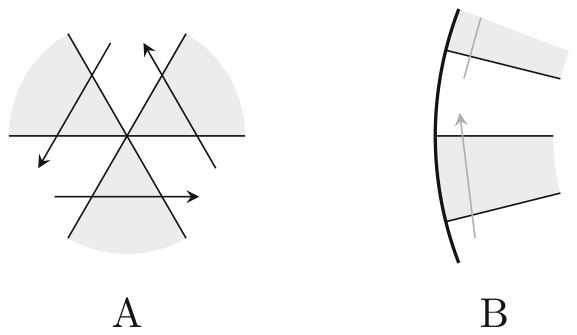
\includegraphics[width=152.3pt]{figs/f1-25.png}
\caption{由 Thurston 图得到的交换矩阵。}
\label{fig:1.25}
\end{figure}

容易验证：交换矩阵在变异 A 下不变，而在变异 B 下按簇的规则改变。这种箭头族连同白面的一个指标列举，其例子见图 1.23 B。从该图可以看出，例如 $\varepsilon^{12}=-1$（有一条从面 2 指向面 1 的实线箭头），而 $\varepsilon^{34}=-1/2$（有一条从 4 指向 3 的实线箭头，以及一条反方向的灰色箭头）。

\begin{figure}[htbp]
\centering
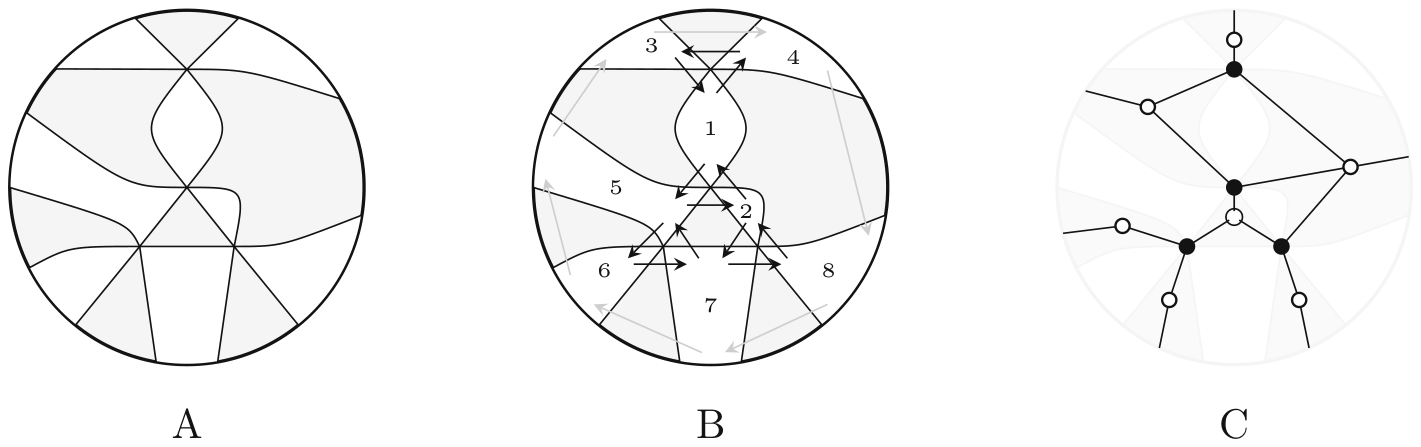
\includegraphics[width=375.1pt]{figs/f1-23.png}
\caption{A：圆盘上的 Thurston 图；B：交换矩阵的构造；C：二部图的构造。}
\label{fig:1.23}
\end{figure}

\textbf{Thurston 图与二部图。}每个 Thurston 图都可以联系上一个二部图。反之，每个白顶点为三价的二部图都对应于一个 Thurston 图。

为从 Thurston 图构造二部图，我们在每个灰面内放一个白顶点，并在边界的每一段灰色段上放一个终止顶点。然后，在每个三重点处放一个黑顶点，并把它与该顶点周围三个面中的三个黑顶点相连。再把终止顶点与相应的白顶点相连。图 1.23 C 给出了与一个 Thurston 图相应的这种图之例。\begin{annote}上句中的第二个“黑顶点”应为“白顶点”：黑顶点放在三重点处，白顶点放在灰面内，故三重点应与三个白顶点相连。底本如此排印，译文照排。[来源：上下文推断]\end{annote}

注意这个对应具有以下性质：
\begin{enumerate}[label=(\roman*),leftmargin=3em,itemsep=1pt]
\item 一个灰色 Thurston 变换对应于两个 A 型 GK 变换（图 1.9）；
\item 一个白色 Thurston 变换对应于 GK 的蛛形变换（C 型，图 1.9）；
\item 二部图的面对应于 Thurston 图的白面；
\item 二部图的之字形路径对应于 Thurston 图的曲线。
\end{enumerate}

\textbf{Thurston 图与三角剖分。}对曲面的任何三角剖分以及任何整数 $N\geqslant 2$，都可以联系上一个 Thurston 图。我们以 $N=2$ 与 $N=3$ 来说明这一构造。

设曲面 $\Sigma$ 被三角剖分，其边或者完全属于边界，或者完全属于内部。把每个三角形替换成 $3(N-1)$ 条曲线，如图 1.26 A（$N=2$）与图 1.26 B（$N=3$）所示；对更大的 $N$ 类似。

\begin{figure}[htbp]
\centering
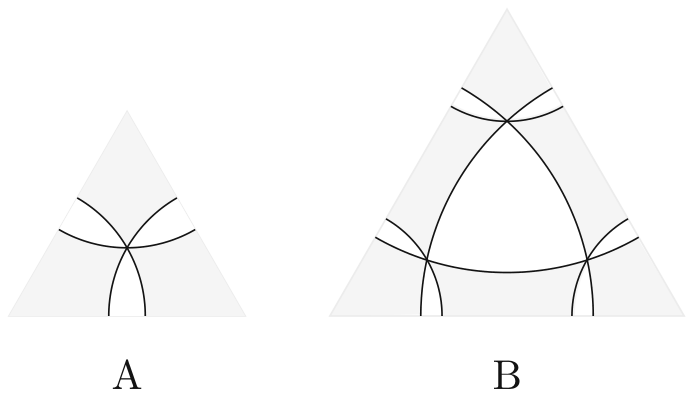
\includegraphics[width=183.0pt]{figs/f1-26.png}
\caption{对应于一个三角形的 Thurston 图，情形 A：$N=2$；B：$N=3$。}
\label{fig:1.26}
\end{figure}

所建立的对应具有以下性质：
\begin{enumerate}[label=(\roman*),leftmargin=3em,itemsep=1pt]
\item 三角剖分的一次翻转对应于一系列 Thurston 变换；当 $N=2$ 时，每次翻转对应于单个 Thurston 变换；
\item 相应的簇代数簇是 $\Sigma$ 上 $\operatorname{SL}(N)$ 局部系统的（带标架的）空间，见 [5]；
\item Thurston 图的每条闭曲线都收缩为围绕一个穿刺点的曲线；
\item 每个穿刺点恰好被 $N-1$ 条曲线围绕；
\item 对偶曲面 $\tilde\Sigma$ 是 $\Sigma$ 的 $N$ 重覆盖，在三重点处分歧。
\end{enumerate}

\textbf{Thurston 图的三元性。}Thurston 图成三出现，使得三元组中的每一个成员都决定另外两个。给定一个 Thurston 图，对每条闭曲线沿其边界粘上一个圆盘，对每条非闭曲线则沿其边界的一半粘上一个圆盘。我们得到一个 CW 复形，其中每个 1-胞腔属于三个 2-胞腔——白色、灰色，以及我们将染成黄色的新圆盘。删去某一类的所有圆盘，就得到其上带有一个 Thurston 图的光滑二维曲面。容易看出，定向相反的黄-灰曲面与初始的（白-灰）曲面对偶。

\textbf{Thurston 图与双置换群。}Thurston 图与双置换群中的词之间的对应具有以下性质：
\begin{enumerate}[label=(\roman*),leftmargin=3em,itemsep=1pt]
\item 关系 $s_is_{i+1}s_i=s_{i+1}s_is_{i+1}$ 以及 $s_{\bar\imath}s_{\overline{\imath+1}}s_{\bar\imath}=s_{\overline{\imath+1}}s_{\bar\imath}s_{\overline{\imath+1}}$ 对应于两个 Thurston 变换的复合，一灰一白（见图 1.27）；
\item 关系 $s_is_{\bar\imath}=s_{\bar\imath}s_i$ 对应于单个白色 Thurston 变换；
\item 关系 $s_is_{\overline{\imath+1}}=s_{\overline{\imath+1}}s_i$ 对应于单个灰色 Thurston 变换；
\item 所有其他外尔群关系只对应于图的同痕；
\item 词的乘积对应于条带的粘合；
\item 不可约词对应于极小的图；
\item 对应于给定词 $s_{i_1}\cdots s_{i_l}$ 的极小 Thurston 图的簇种子，与对应于该词的簇种子同构。
\end{enumerate}

\begin{figure}[htbp]
\centering
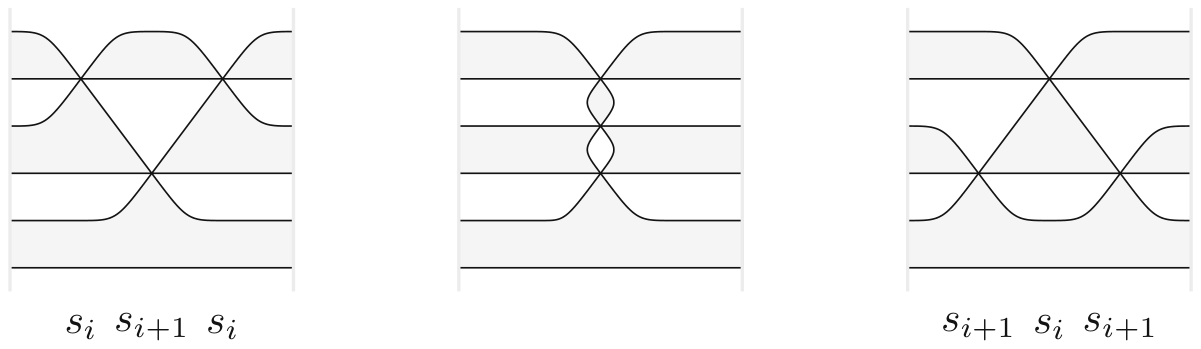
\includegraphics[width=317.1pt]{figs/f1-27.png}
\caption{对应于关系 $s_is_{i+1}s_i=s_{i+1}s_is_{i+1}$ 的 Thurston 变换。}
\label{fig:1.27}
\end{figure}

\textbf{Thurston 图与余扩张双仿射外尔群。}对于群 $\widehat{\operatorname{PGL}}(N)$，§1.4.1 中给出的外尔群之双拷贝的余扩张 $(W\times W)^{\sharp}$ 对应于柱面上的一个 Thurston 图，我们把它水平地画出。与前一种情形一样，每个图由 $2N$ 条没有竖直切线的曲线组成，从左边走到右边。表示 $s_i$ 与 $s_{\bar\imath}$（$i\neq0$）的图与有限情形同样构造。$s_0$ 与 $s_{\bar0}$ 的图分别对应于曲线 $2N-1,2N,1$ 与 $2N,1,2$ 的三重点。生成元 $\Lambda$ 由没有交点、但把柱面左端的第 $i$ 个点与右端的第 $i-2\pmod N$ 个点相连的图表示。这种对应的性质表与有限情形相同。

\textbf{Thurston 图与链环图。}对曲面 $\Sigma$ 上的每个纽结或链环图，都可以按照图 1.28 所示的规则联系上 Thurston 图。按照定向的不同，这可以用两种方式进行。

\begin{figure}[htbp]
\centering
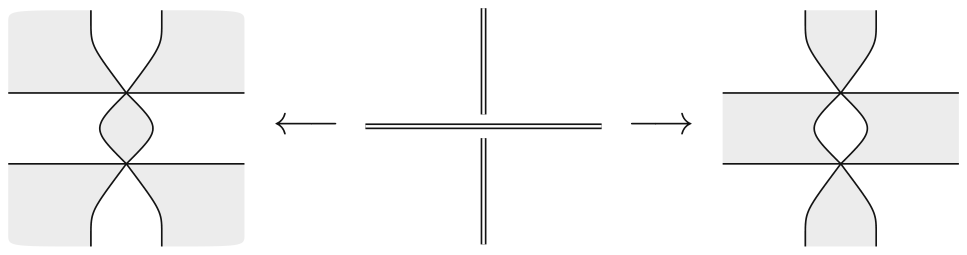
\includegraphics[width=255.3pt]{figs/f1-28.png}
\caption{对应于链环图的 Thurston 图。}
\label{fig:1.28}
\end{figure}

这个对应具有以下性质：
\begin{enumerate}[label=(\roman*),leftmargin=3em,itemsep=1pt]
\item 把图上的一个上穿改成下穿，对应于一个 Thurston 变换；
\item 第一种 Thurston 图的白面对应于链环图中交叉点之间的线段；
\item 第二种 Thurston 图的白面对应于纽结图的面以及交叉点；
\item 链环图的 Reidemeister-III 变换对应于四个灰色与四个白色 Thurston 变换的复合；这个变换对应于
\[
s_is_{\bar\imath}s_{i+1}s_{\overline{\imath+1}}s_is_{\bar\imath}\to s_{i+1}s_{\overline{\imath+1}}s_is_{\bar\imath}s_{i+1}s_{\overline{\imath+1}};
\]
\item Reidemeister-II 变换对应于一个灰色与一个白色 Thurston 变换，以及两个灰色与两个白色 Thurston 约化；
\item Reidemeister-I 变换对应于一个灰色与一个白色 Thurston 约化；
\item 亏格为 $g$ 的曲面上的链环图所对应的二部图，其白顶点比黑顶点多 $2g-2$ 个。
\end{enumerate}

本段的一个本质部分，是把 Cohen、Dasbach 与 Russell 在 [3] 中所作的构造翻译成 Thurston 图的语言。

\section{附录 E：子式生成函数的性质的证明}

首先，我们证明生成函数的卷积给出矩阵乘积的生成函数。采用矩阵记号，把行（相应地，列）记作 $\xi$ 与 $\xi'$（相应地，$\eta$ 与 $\eta'$），我们得到
\begin{gather*}
\int S(M_1,\xi',\eta)S(M_2,\xi,\eta')e^{-\xi\eta}\,d\xi\,d\eta
=\int \exp\left(\xi'M_1\eta+\xi M_2\eta'-\xi\eta\right)d\xi\,d\eta\\
=\int \exp\left(-(\xi-\xi'M_1)(\eta-M_2\eta')+\xi'M_1M_2\eta'\right)d\xi\,d\eta\\
=\exp\left(\xi'M_1M_2\eta'\right)\int \exp\left(-\xi\eta\right)d\xi\,d\eta
=\exp\left(\xi'M_1M_2\eta'\right),
\end{gather*}
其中
\[
d\xi\,d\eta=\prod_{j=1}^n d\xi_j\,d\eta^j=d\xi_1\cdots d\xi_n\,d\eta^n\cdots d\eta^1.
\]

其次，我们证明表达式 $\exp\left(\xi M\eta\right)$ 确实是矩阵的子式的生成函数，正如引理 1.5.2(ii) 所述：
\begin{align*}
\exp\left(\sum_{i,j} M_j^i\xi_i\eta^j\right)
&=\sum_{k=0}^n\frac1{k!}\sum_{\substack{i_1,\dots,i_k\\ j_1,\dots,j_k}}M_{j_1}^{i_1}\cdots M_{j_k}^{i_k}\,\xi_{i_1}\eta^{j_1}\cdots\xi_{i_k}\eta^{j_k}\\
&=\sum_{k=0}^n\sum_{\substack{i_1<\cdots<i_k\\ j_1,\dots,j_k}}M_{j_1}^{i_1}\cdots M_{j_k}^{i_k}\,\xi_{i_1}\eta^{j_1}\cdots\xi_{i_k}\eta^{j_k}\\
&=\sum_{k=0}^n(-1)^{\frac{k(k-1)}2}\sum_{\substack{i_1<\cdots<i_k\\ j_1,\dots,j_k}}M_{j_1}^{i_1}\cdots M_{j_k}^{i_k}\,\xi_{i_1}\cdots\xi_{i_k}\eta^{j_1}\cdots\eta^{j_k}\\
&=\sum_{k=0}^n(-1)^{\frac{k(k-1)}2}\sum_{\substack{i_1<\cdots<i_k\\ j_1<\cdots<j_k}}\sum_{\sigma\in\mathfrak{S}_k}M_{j_{\sigma(1)}}^{i_1}\cdots M_{j_{\sigma(k)}}^{i_k}\,\xi_{i_1}\cdots\xi_{i_k}\eta^{j_{\sigma(1)}}\cdots\eta^{j_{\sigma(k)}}\\
&=\sum_{k=0}^n(-1)^{\frac{k(k-1)}2}\sum_{\substack{i_1<\cdots<i_k\\ j_1<\cdots<j_k}}\sum_{\sigma\in\mathfrak{S}_k}(-1)^{\operatorname{sign}(\sigma)}M_{j_{\sigma(1)}}^{i_1}\cdots M_{j_{\sigma(k)}}^{i_k}\,\xi_{i_1}\cdots\xi_{i_k}\eta^{j_1}\cdots\eta^{j_k}\\
&=\sum_{k=0}^n(-1)^{\frac{k(k-1)}2}\sum_{\substack{i_1<\cdots<i_k\\ j_1<\cdots<j_k}}M_{j_1,\dots,j_k}^{i_1,\dots,i_k}\,\xi_{i_1}\cdots\xi_{i_k}\eta^{j_1}\cdots\eta^{j_k}\\
&=\sum_{k=0}^n\sum_{\substack{i_1<\cdots<i_k\\ j_1<\cdots<j_k}}M_{j_1,\dots,j_k}^{i_1,\dots,i_k}\,\xi_{i_1}\cdots\xi_{i_k}\eta^{j_k}\cdots\eta^{j_1}.
\end{align*}

\section{附录 F：Schwartz 坐标与五角星映射}

为简化记号，我们把指标 $i+k$ 换成 $k$ 个撇号。在新记号下，规范化条件 (1.44) 写为 $e'''=a(e'+e)+be''$。先看下面的恒等式：
\[
a(e'+e)-be'=\frac{a'+bb'}{a'}e'''-\frac{b}{a'}e''''.
\]
事实上，我们有 $a(e'+e)=e'''-be''$ 与 $a'(e''+e')=e''''-b'e'''$。第二个等式给出
\[
e'=\frac{e''''-b'e'''-a'e''}{a'}.
\]
于是，把右端用 $e''$、$e'''$ 与 $e''''$ 表示出 $e$ 与 $e'$，便得到上述恒等式。

这个恒等式表明，$a(e'+e)-be'$ 对应于交点 $(p,p')\cap(p'',p''')$。略微滥用记号，把向量与射影平面上相应的点等同起来，就有
\begin{equation}
\begin{aligned}
x&=\left[e,e',e'+e,a(e'+e)-be'\right]
 =\left[0,\infty,1,1-\frac ba\right] =\frac ba,\\
y&=\left[e'''',e''',e''''-b'e''',(a'+bb')e'''-be''''\right]
 =\left[0,\infty,-b',-b'-\frac{a'}{b}\right] =-\frac{a'}{bb'}.
\end{aligned}
\tag{1.58}\label{eq:1.58}
\end{equation}
反过来，$a=-(xx'y)^{-1}$、$b=-(x'y)^{-1}$；或者恢复原来的指标，最终得到公式 (1.46) 与 (1.47)。

现在考虑五角星映射。在简化记号下，演化后的向量及其规范化条件写为
\[
\tilde e=\alpha(e+e'),\qquad
\tilde e'''=\tilde a(\tilde e+\tilde e')+\tilde b\tilde e''.
\]
把第一个等式代入第二个，得到
\[
\alpha'''(e''''+e''')=\alpha\tilde a(e'+e)+\alpha'\tilde a(e''+e')+\alpha''\tilde b(e'''+e'').
\]
考虑到关系 (1.44)，即 $e'''=a(e'+e)+be''$，可以消去 $e$ 与 $e'$：
\[
\alpha'''(e''''+e''')=\frac{\alpha\tilde a}{a}(e'''-be'')+\frac{\alpha'\tilde a}{a'}(e''''-b'e''')+\alpha''\tilde b(e'''+e'').
\]
于是，在设 $e''''$、$e'''$ 与 $e''$ 线性无关之后，我们得到由三个方程组成的方程组
\[
0=-\frac{\alpha b\tilde a}{a}+\alpha''\tilde b,\qquad
\alpha'''=\frac{\alpha\tilde a}{a}-\frac{\alpha'b'\tilde a}{a'}+\alpha''\tilde b,\qquad
\alpha'''=\frac{\alpha'\tilde a}{a'}.
\]
由此，一方面得到
\[
\alpha\frac{1+b}{a}=\alpha'\frac{1+b'}{a'},
\]
另一方面得到 $\alpha=ca/(1+b)$。把第一式代入第二式，便得到 $\tilde a$ 与 $\tilde b$ 的表达式：
\[
\tilde a=\frac{a'''(b'+1)}{b'''+1},\qquad
\tilde b=\frac{a'''b(b'+1)(b''+1)}{a''(b+1)(b'''+1)}.
\]
现在，与 (1.51) 类似，Schwarz 坐标变换的一个直接计算给出
\[
\tilde x=x''\frac{1-x'''y''}{1-x'y},\qquad
\tilde y=y'\frac{1-x'y}{1-x'''y''},
\]
它正是五角星映射。

最后，由方程 (1.52)，可以把解 (1.53) 写成
\[
\tilde u'=v^{-1},\qquad
\tilde v=u''\frac{(1+v)(1+v''')}{(1+v'^{-1})(1+v''^{-1})},
\]
其中 $u'=-(xy)^{-1}$、$v=-x'y$。这正是公式 (1.55)。
